\chapter{Integración de Sistemas}
En este capítulo, se aborda la fase de integración del sistema. Previamente, en el diseño e implementación, se llevaron a cabo diseños, simulaciones y PCB asociadas a las etapas que componen el sistema de energía desarrollado en este trabajo de investigación. En este punto, se busca integrar cada una de las etapas, siguiendo la lógica funcional establecida en la arquitectura del sistema. Se alcanza un nivel de conexiones físicas mediante el desarrollo de esquemáticos y, finalmente, el diseño de dos PCB de 12x8 cm, de acuerdo con los requisitos estructurales inicialmente definidos en los requerimientos.

\hspace{1.27cm}Adicionalmente, se aborda la integración a nivel de software mediante un flujograma que describe la lógica de programación requerida para la operación del sistema (ver Fig. \ref{fig:flujograma_EPS})

\hspace{1.27cm}Como resultado, obtenemos esquemáticos, los cuales se han dividido en cinco partes (Fig.\ref{fig:EPS_Sheet1} a Fig. \ref{fig:EPS_Sheet5}) y PCB del Sistema (ver Fig. \ref{fig:EPS_Final1} a Fig. \ref{fig:EPS_Final4}), integrando cada una de sus etapas, a nivel de hardware y software.


\newpage


\section{Software}

\begin{figure}[h]
  \centering
  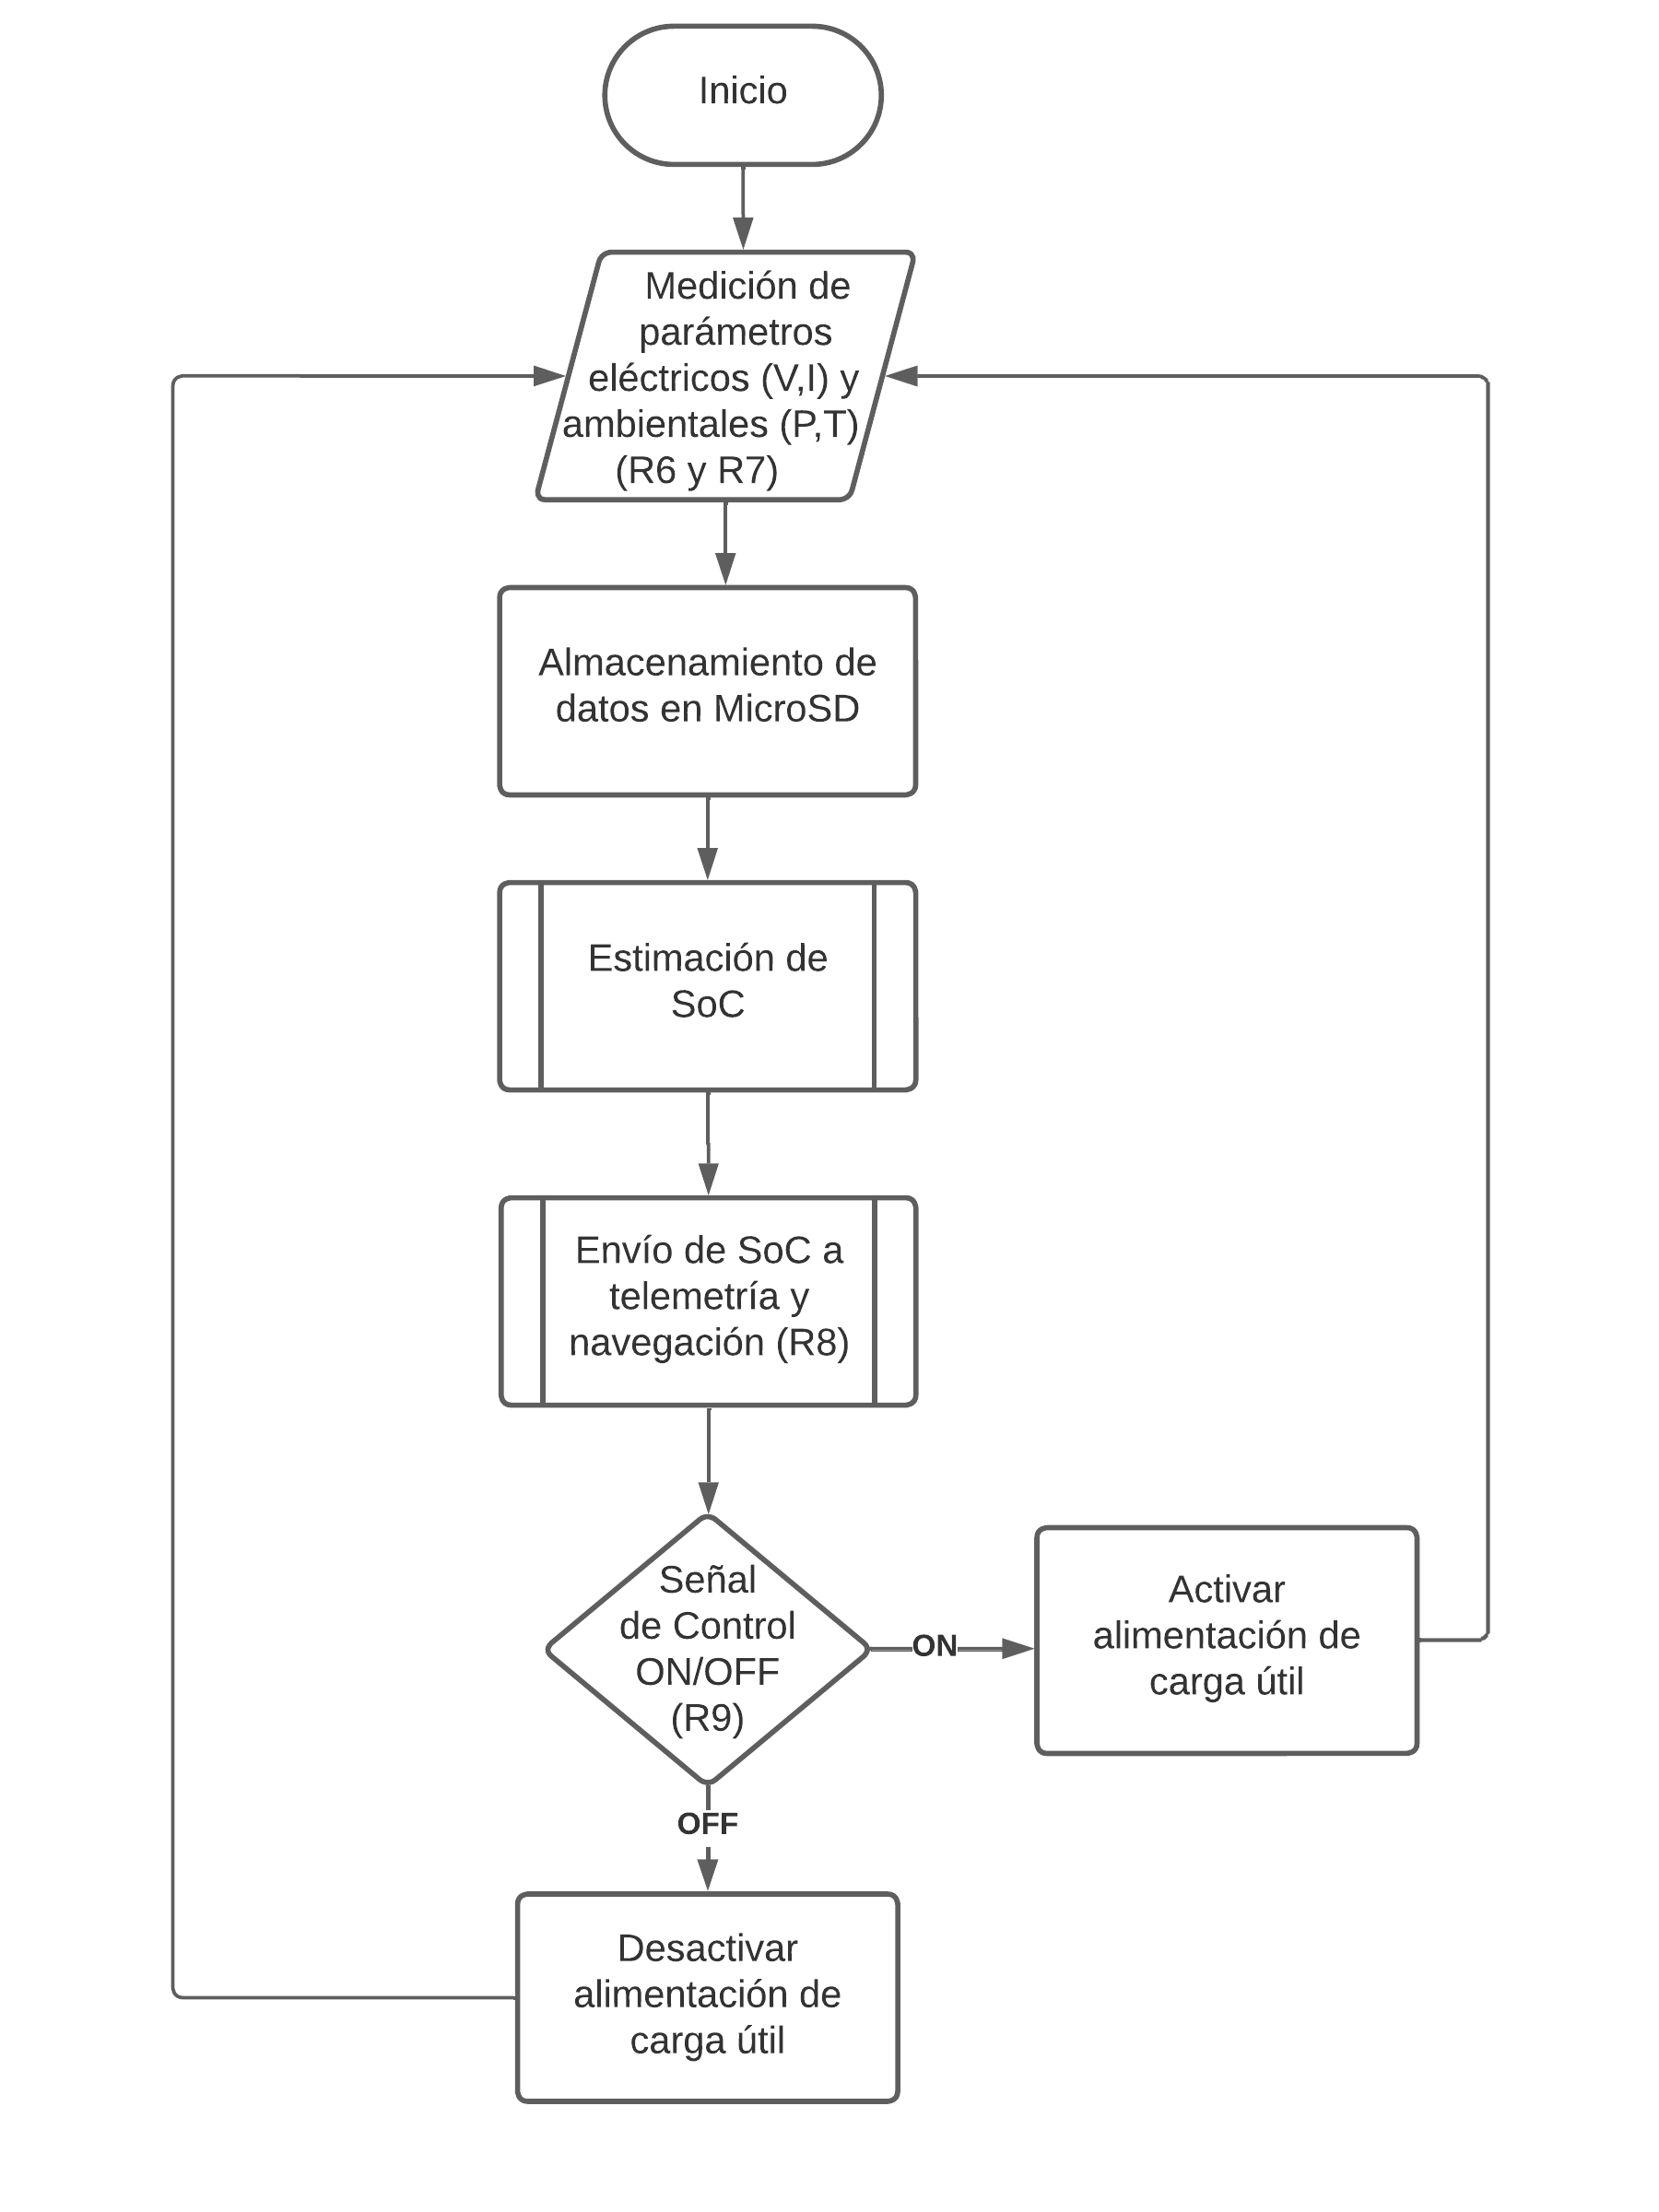
\includegraphics[width=\textwidth]{Pictures/Flujograma_EPS.png}
  \caption{Flujograma de algoritmo de programación para EPS}
  \label{fig:flujograma_EPS}
\end{figure}

\newpage





\section{Hardware}

\begin{figure}[h]
  \centering
  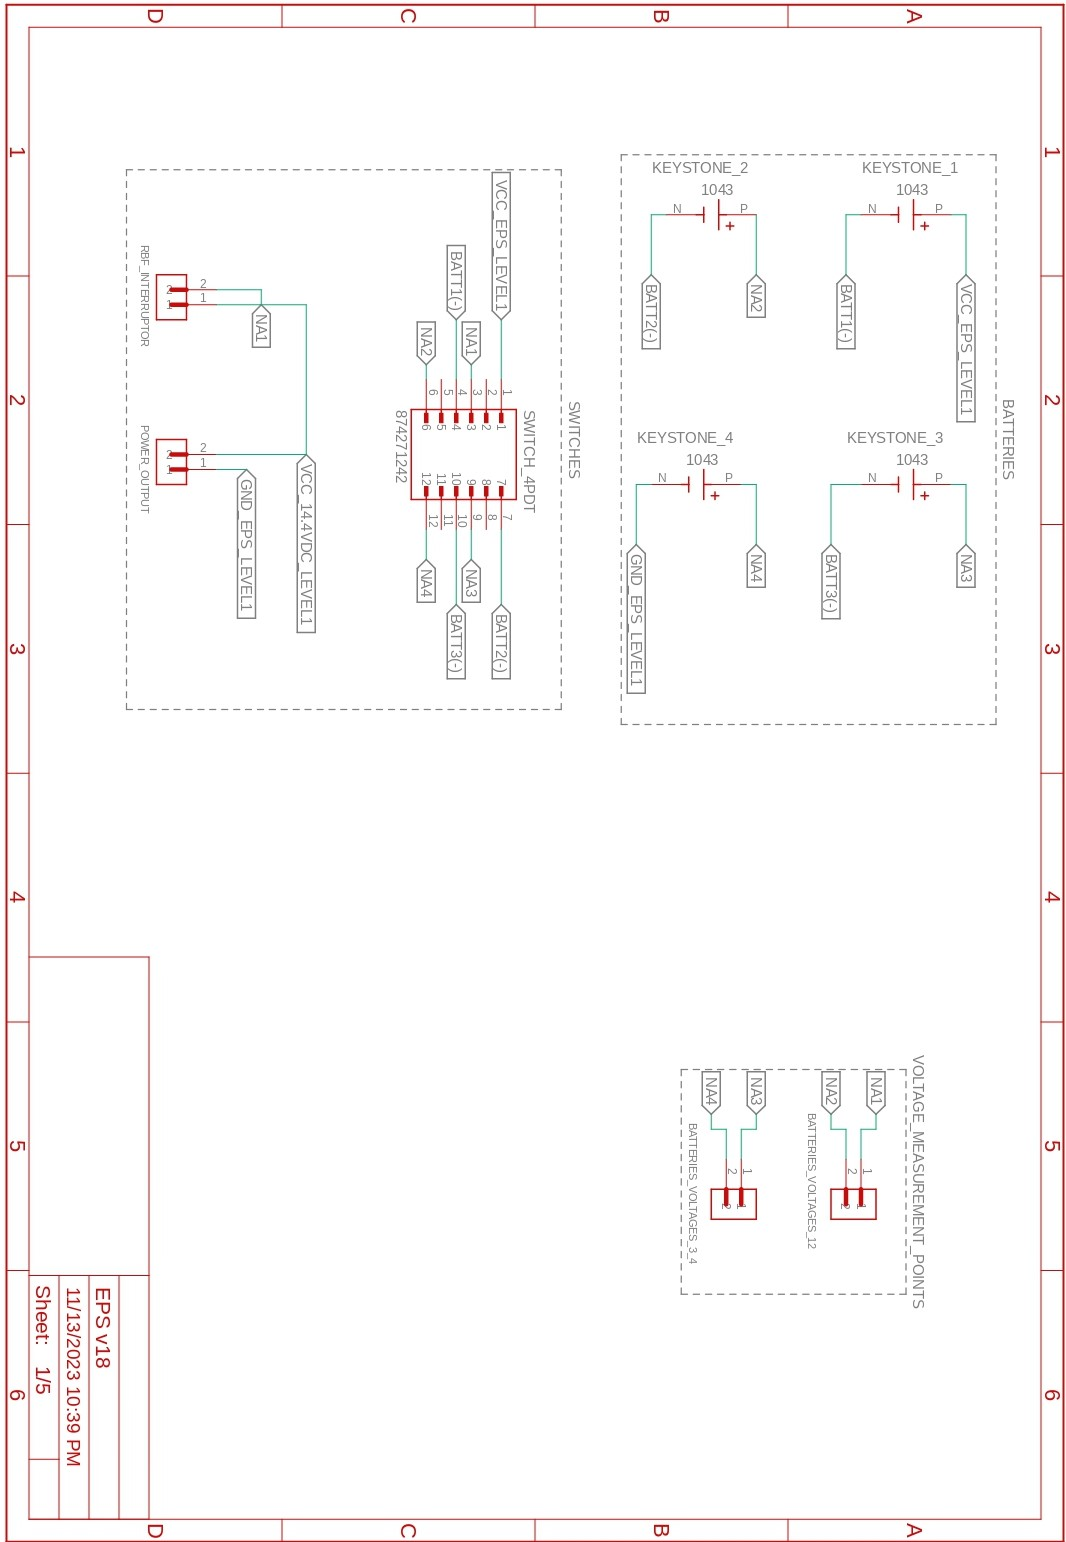
\includegraphics[width=0.955\textwidth]{Pictures/EPS_Sheets_page-0001.jpg}
  \caption{Esquemático de EPS Integrado, Parte I.}
  \label{fig:EPS_Sheet1}
\end{figure}
\newpage

\begin{figure}[h]
  \centering
  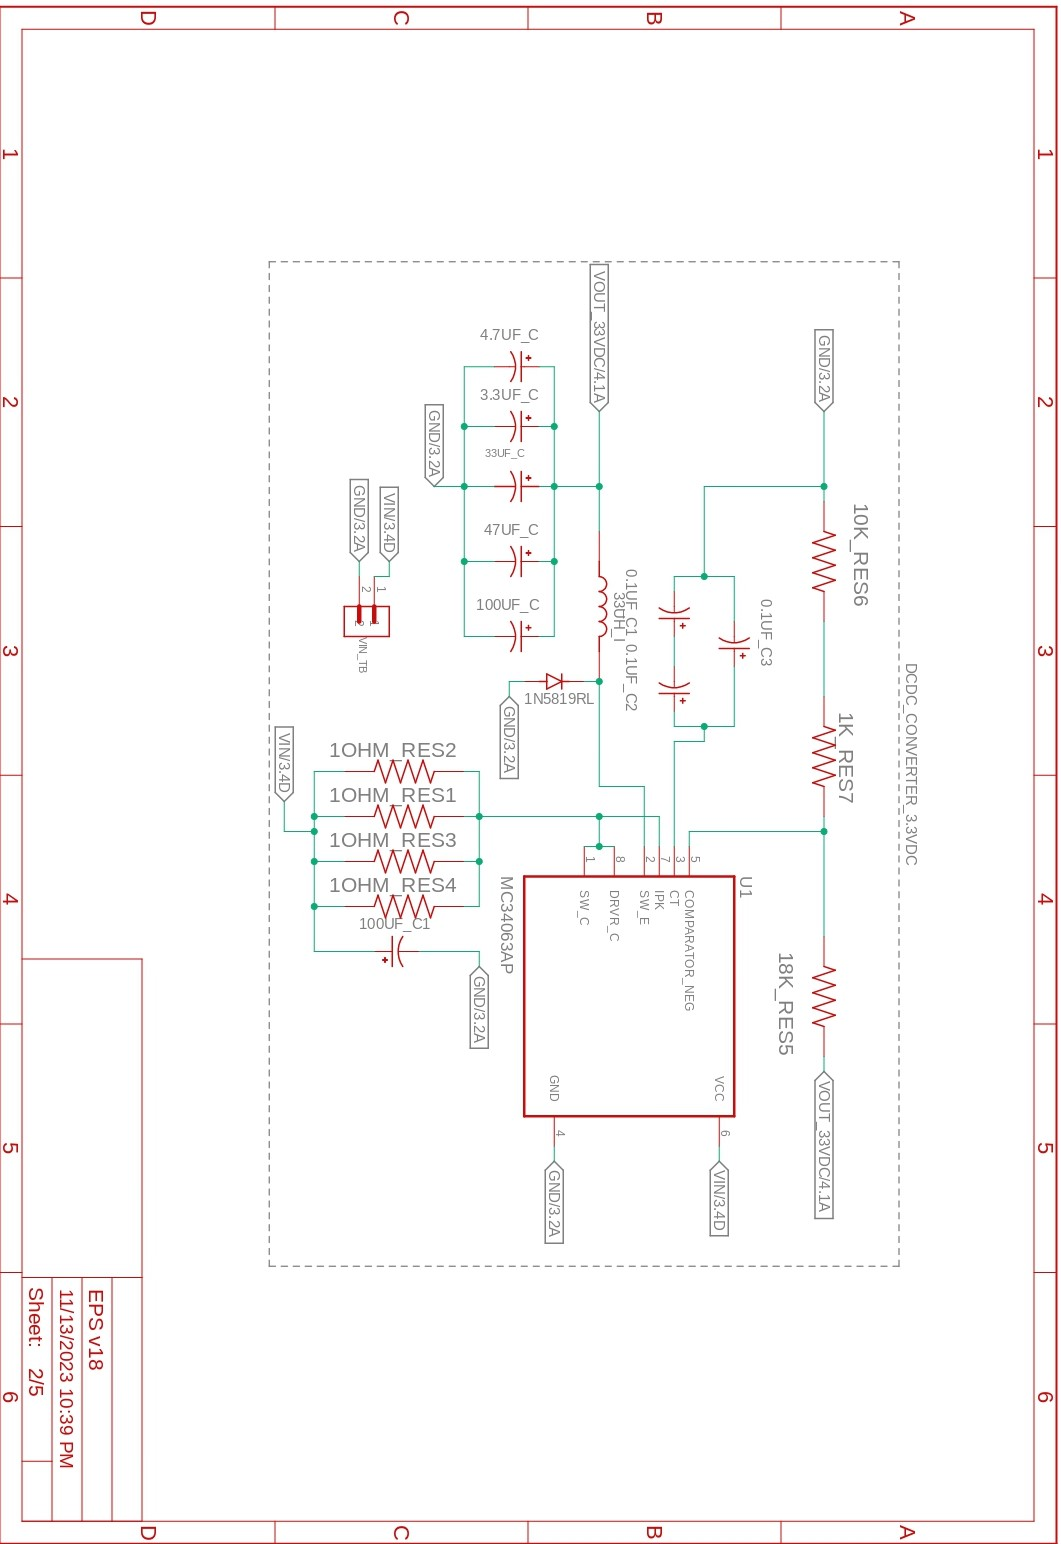
\includegraphics[width=\textwidth]{Pictures/EPS_Sheets_page-0002.jpg}
  \caption{Esquemático de EPS Integrado, Parte II.}
  \label{fig:EPS_Sheet2}
\end{figure}
\newpage
\begin{figure}[h]
  \centering
  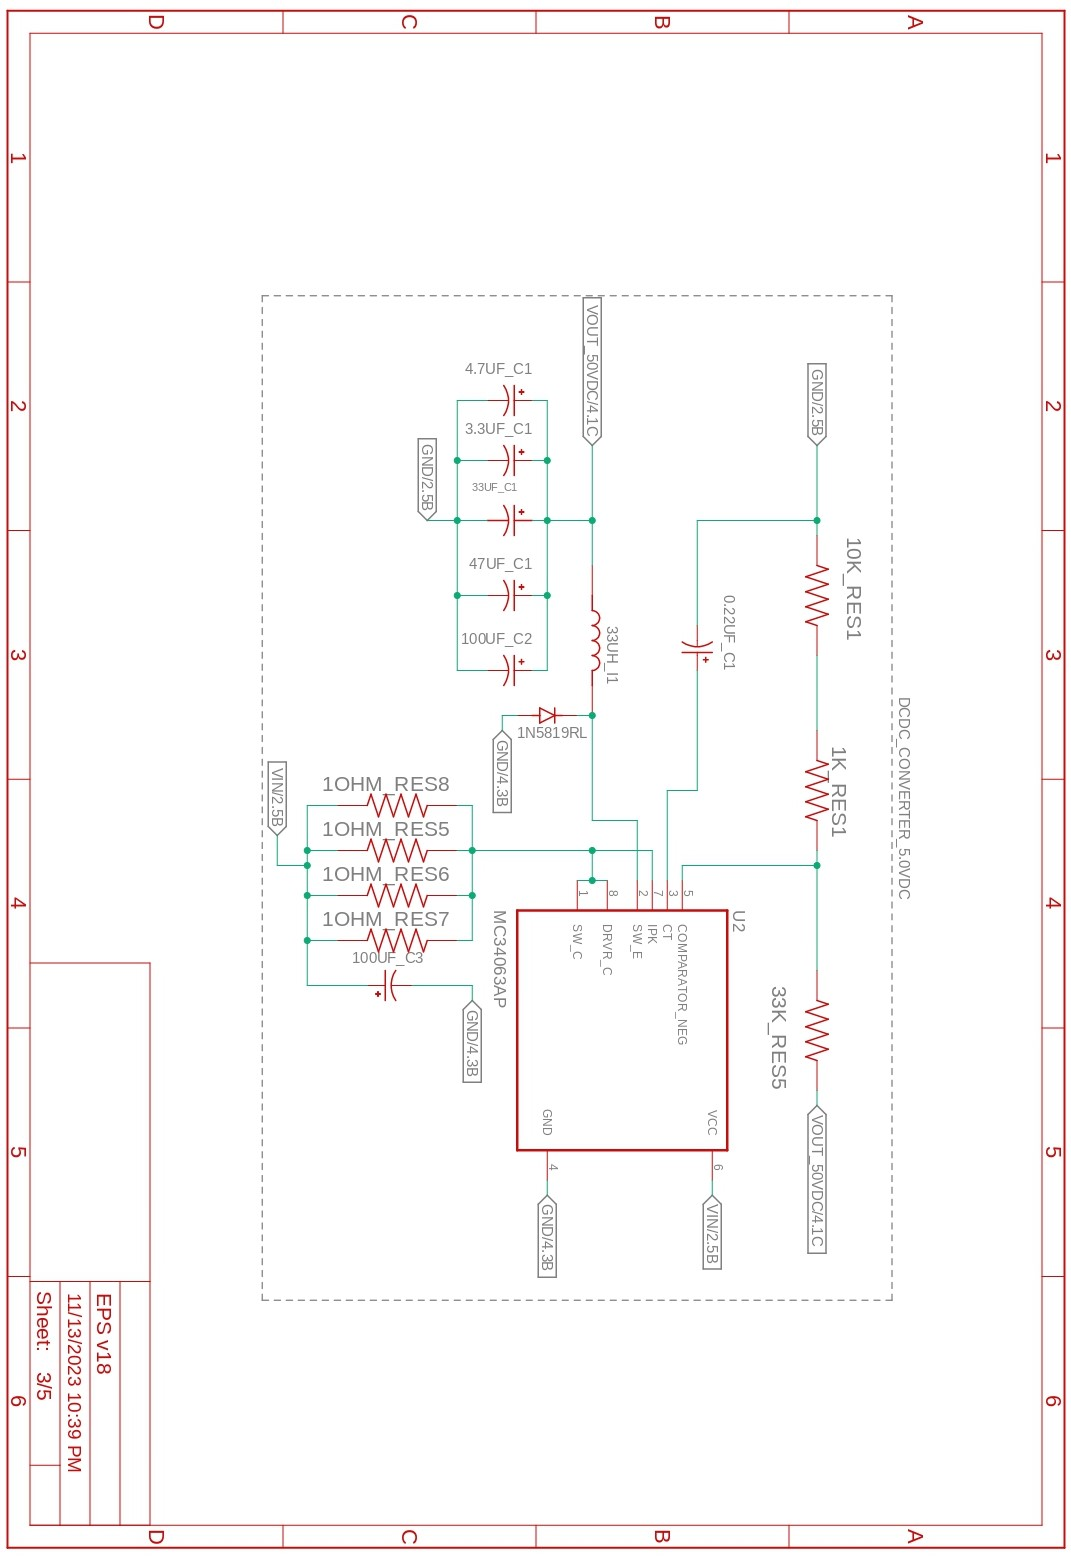
\includegraphics[width=\textwidth]{Pictures/EPS_Sheets_page-0003.jpg}
  \caption{Esquemático de EPS Integrado, Parte III.}
  \label{fig:EPS_Sheet3}
\end{figure}

\newpage
\begin{figure}[h]
  \centering
  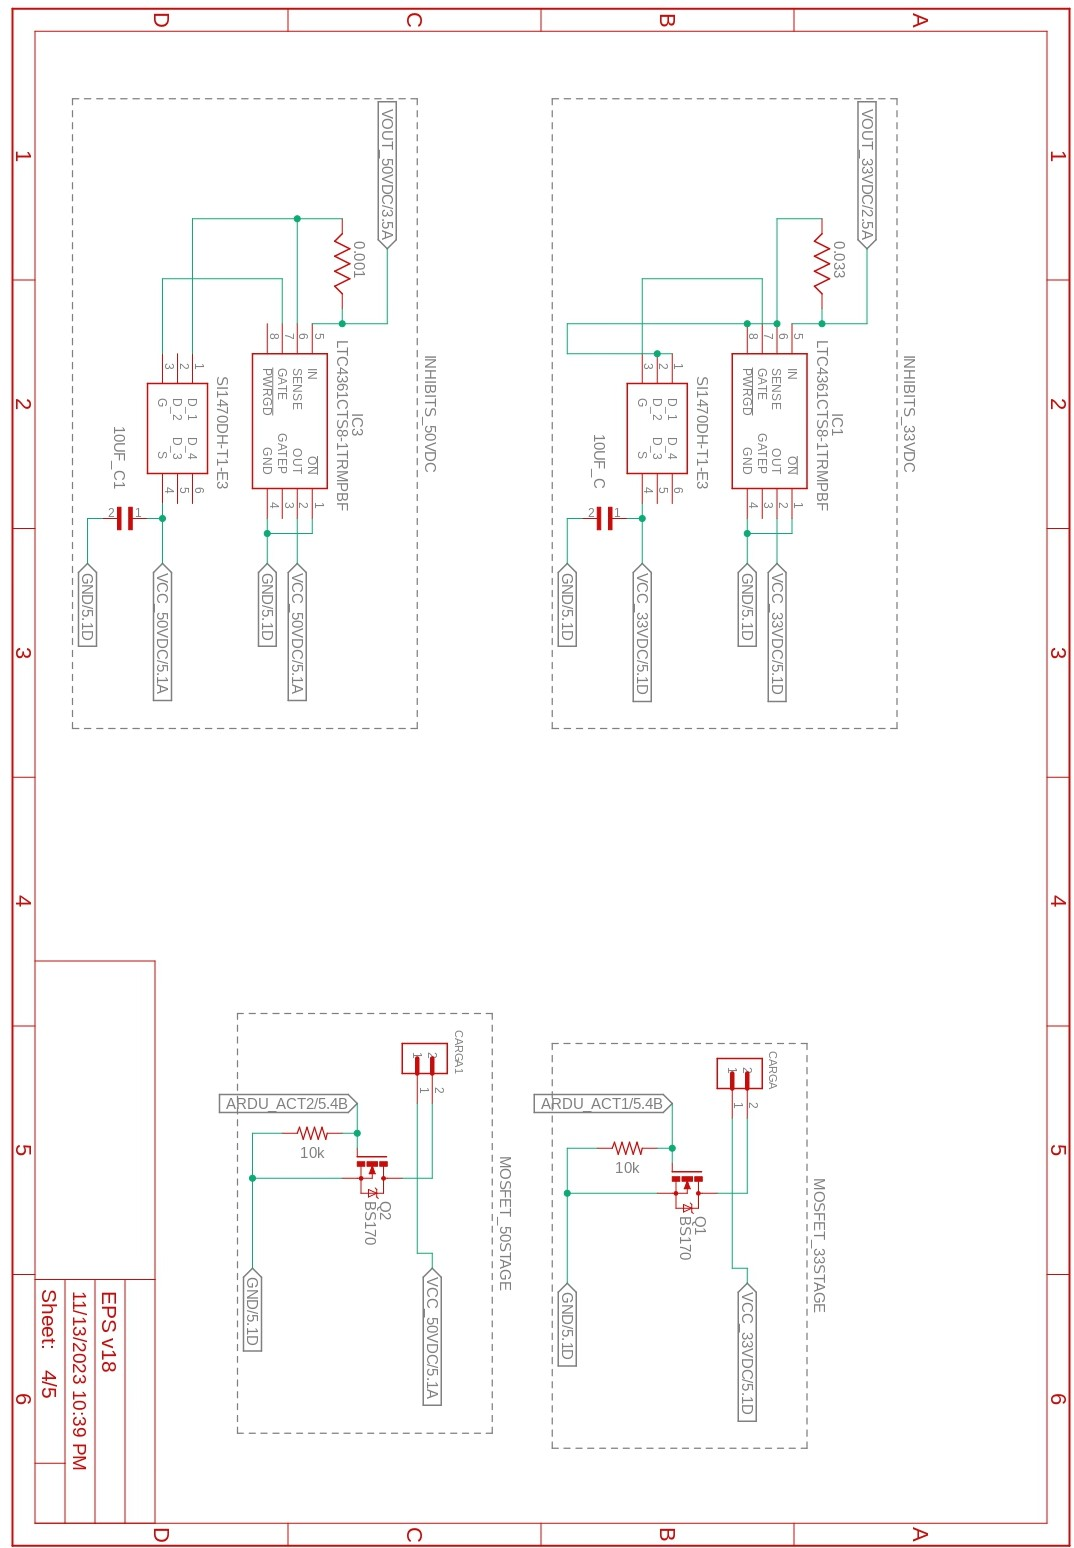
\includegraphics[width=\textwidth]{Pictures/EPS_Sheets_page-0004.jpg}
  \caption{Esquemático de EPS Integrado, Parte IV.}
  \label{fig:EPS_Sheet4}
\end{figure}

\newpage
\begin{figure}[h]
  \centering
  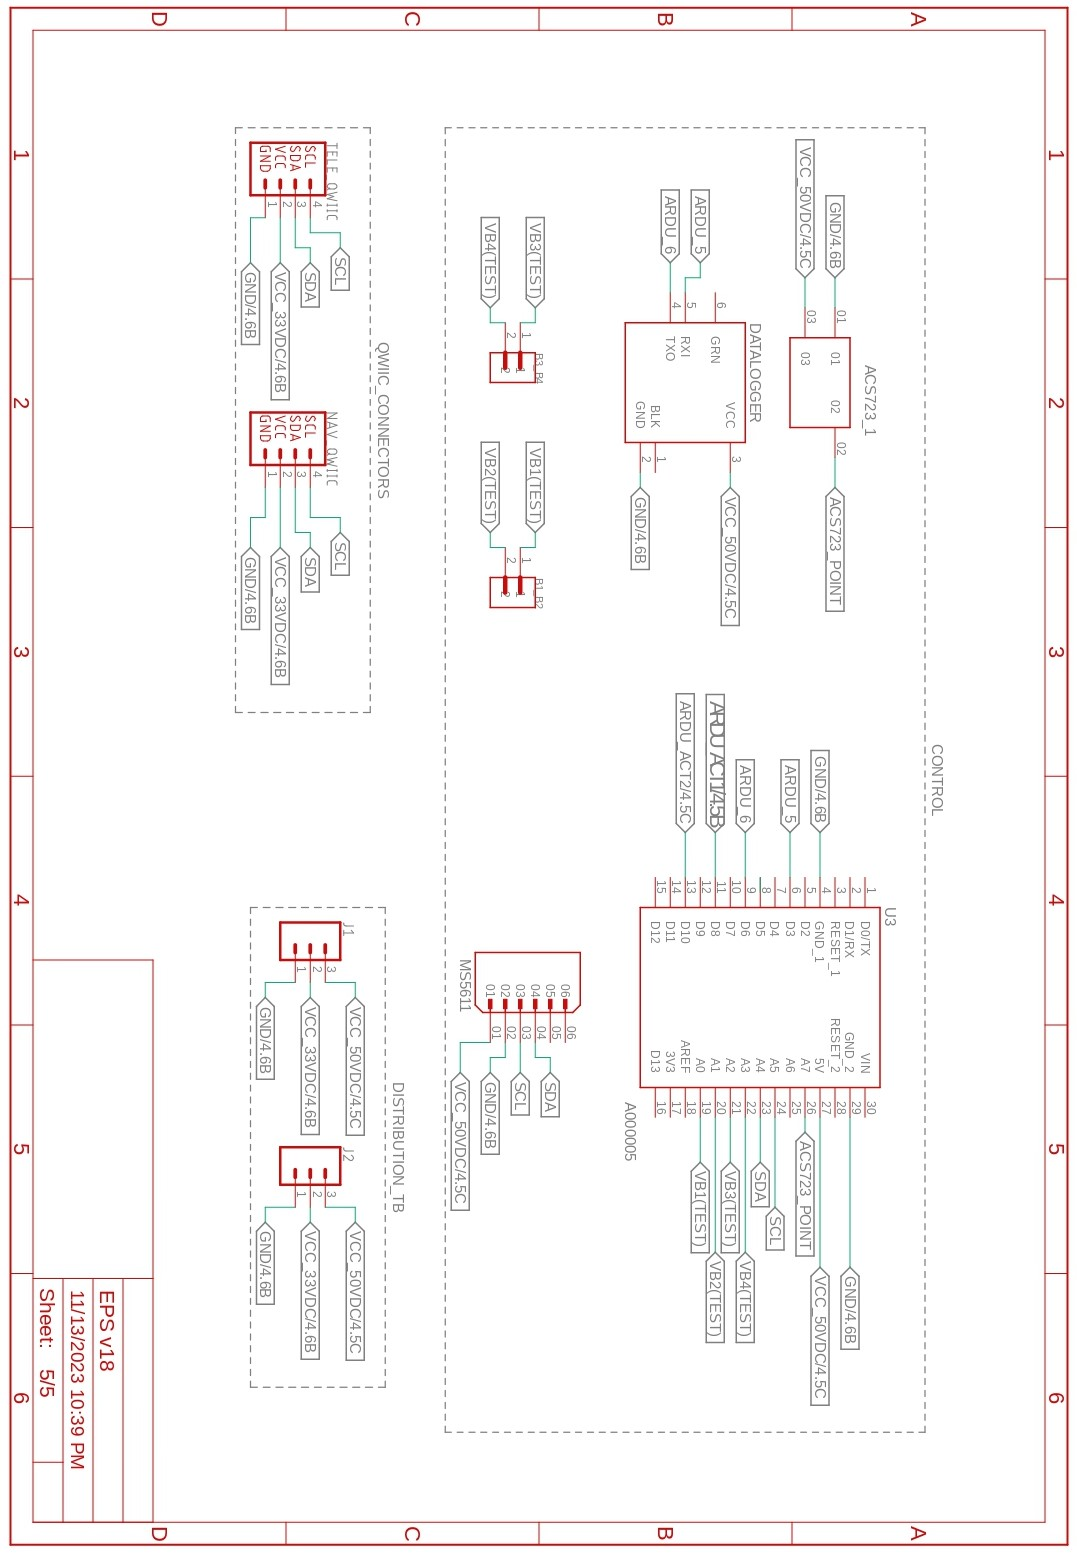
\includegraphics[width=\textwidth]{Pictures/EPS_Sheets_page-0005.jpg}
  \caption{Esquemático de EPS Integrado, Parte V.}
  \label{fig:EPS_Sheet5}
\end{figure}

\newpage
\begin{figure}[h]
  \centering
  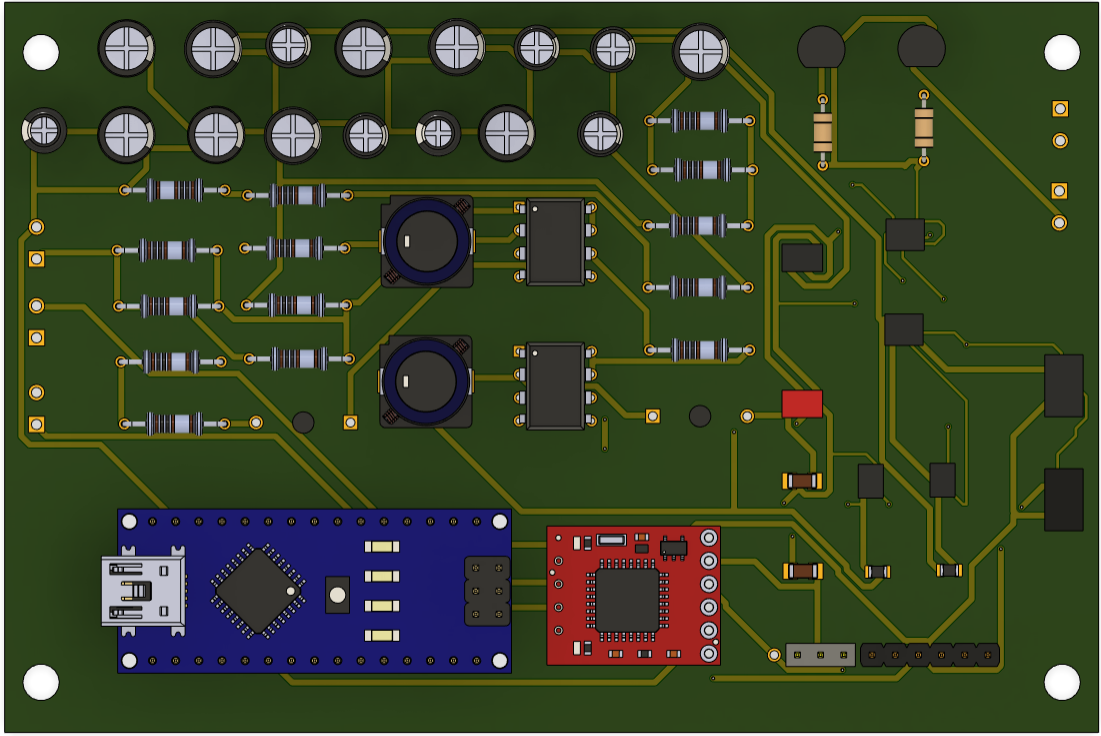
\includegraphics[width=\textwidth]{Pictures/EPS_FINAL.png}
  \caption{Vista frontal 3D de PCB 1 del EPS.}
  \label{fig:EPS_Final1}
\end{figure}

\begin{figure}[h]
  \centering
  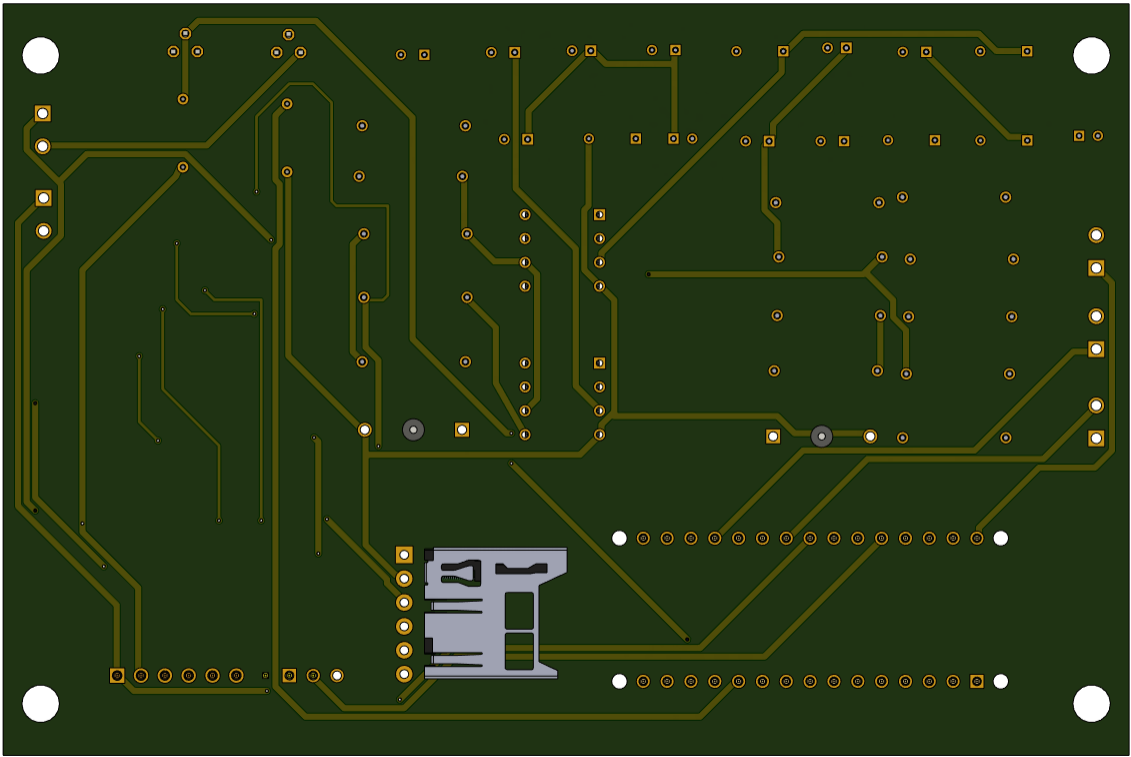
\includegraphics[width=\textwidth]{Pictures/EPS_FINAL2.png}
  \caption{Vista trasera 3D de PCB 1 del EPS.}
  \label{fig:EPS_Final2}
\end{figure}
\newpage

\begin{figure}[h]
  \centering
  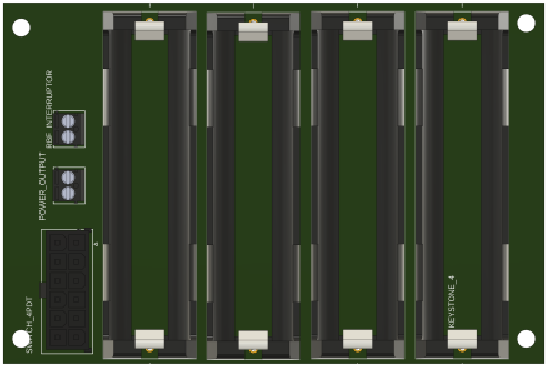
\includegraphics[width=\textwidth]{Pictures/EPS_FINAL4.png}
  \caption{Vista frontal 3D de PCB 2 del EPS.}
  \label{fig:EPS_Final3}
\end{figure}

\begin{figure}[h]
  \centering
  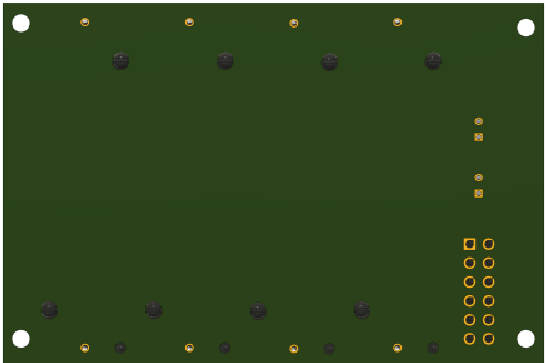
\includegraphics[width=\textwidth]{Pictures/EPS_FINAL3.png}
  \caption{Vista trasera 3D de PCB 2 del EPS.}
  \label{fig:EPS_Final4}
\end{figure}
\newpage


